\documentclass[aspectratio=169]{beamer}

% Packages
\usepackage[utf8]{inputenc}
\usepackage[T1]{fontenc}
\usepackage{amsmath,amssymb}
\usepackage{graphicx}
\usepackage{booktabs}
\usepackage{multirow}
\usepackage{xcolor}
\usepackage{tikz}
\usepackage{hyperref}

% Graphics paths for figures
\graphicspath{{docs/figures/}{models/overnight_full/}{models/lead_specific_v1/}}

% Beamer theme
\usetheme{Madrid}
\usecolortheme{default}

% Custom colors
\definecolor{physicsblue}{RGB}{30, 90, 180}
\definecolor{dlred}{RGB}{180, 50, 50}
\definecolor{successgreen}{RGB}{34, 139, 34}

% Title information
\title[ECG Lead Reconstruction]{12-Lead ECG Reconstruction from 3 Leads:\\A Physics-Informed Deep Learning Approach}
\subtitle{DATA 5000 Final Project}
\author{Mithun Manivannan \and Daniel Oladele}
\institute{School of Computer Science\\Carleton University}
\date{December 2025}

\begin{document}

% =============================================================================
% TITLE SLIDE
% =============================================================================
\begin{frame}
    \titlepage
\end{frame}

% =============================================================================
% OUTLINE
% =============================================================================
\begin{frame}{Outline}
    \tableofcontents
\end{frame}

% =============================================================================
% SECTION 1: THE PROBLEM
% =============================================================================
\section{Clinical Motivation}

\begin{frame}{Cardiovascular Disease: A Global Health Crisis}
    \begin{columns}[c]
        \column{0.55\textwidth}
        \begin{itemize}
            \item \textbf{17.9 million deaths annually} from cardiovascular disease (WHO, 2023)
            \item Leading cause of death globally: \textbf{32\% of all deaths}
            \item \textbf{80\% of premature CVD deaths are preventable} with early detection
            \item The \textbf{12-lead ECG} remains the gold standard for cardiac diagnosis
        \end{itemize}
        
        \vspace{0.3cm}
        \begin{block}{Research Question}
            Can we accurately reconstruct a full 12-lead ECG from only 3 input leads, enabling clinical-grade cardiac diagnosis from portable devices?
        \end{block}
        
        \column{0.42\textwidth}
        \begin{figure}
            \centering
            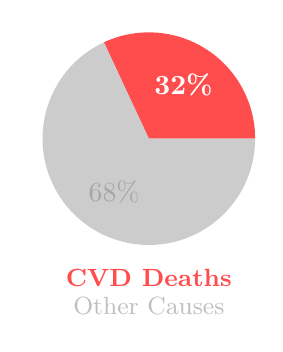
\begin{tikzpicture}[scale=0.9]
                % Pie chart showing CVD deaths
                \fill[red!70] (0,0) -- (0:1.5) arc (0:115:1.5) -- cycle;
                \fill[gray!40] (0,0) -- (115:1.5) arc (115:360:1.5) -- cycle;
                \node[white, font=\bfseries] at (57:0.9) {32\%};
                \node[gray!70] at (237:0.9) {68\%};
                \node[below, red!70, font=\small\bfseries] at (0,-1.7) {CVD Deaths};
                \node[below, gray!50, font=\small] at (0,-2.1) {Other Causes};
            \end{tikzpicture}
            \caption{Global mortality distribution (WHO, 2023)}
        \end{figure}
    \end{columns}
\end{frame}

\begin{frame}{The 12-Lead ECG: Anatomy and Clinical Significance}
    \begin{columns}[c]
        \column{0.5\textwidth}
        \textbf{Standard 12-Lead Configuration:}
        \begin{itemize}
            \item \textcolor{physicsblue}{\textbf{Limb leads} (6)}: I, II, III, aVR, aVL, aVF
            \begin{itemize}
                \item View heart in frontal plane
                \item Related by Einthoven's and Goldberger's laws
            \end{itemize}
            \item \textcolor{dlred}{\textbf{Chest leads} (6)}: V1--V6
            \begin{itemize}
                \item View heart in transverse plane
                \item No deterministic relationships
            \end{itemize}
        \end{itemize}
        
        \vspace{0.2cm}
        \textbf{Electrode Requirements:}
        \begin{itemize}
            \item Standard: \textbf{10 electrodes} (4 limb + 6 chest)
            \item Our approach: \textbf{4 electrodes} (RA, LA, LL, V4)
        \end{itemize}
        
        \column{0.48\textwidth}
        \begin{figure}
            \centering
            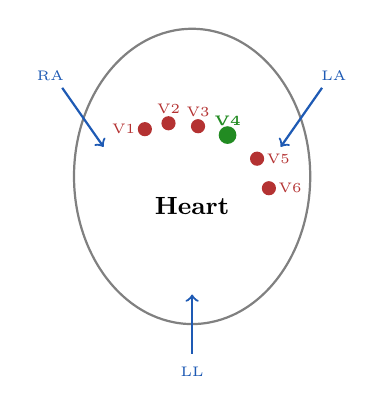
\begin{tikzpicture}[scale=0.75]
                % Torso outline
                \draw[thick, gray] (0,0) ellipse (2 and 2.5);
                
                % V1-V6 positions on chest
                \fill[dlred] (-0.8, 0.8) circle (0.12) node[left, font=\tiny] {V1};
                \fill[dlred] (-0.4, 0.9) circle (0.12) node[above, font=\tiny] {V2};
                \fill[dlred] (0.1, 0.85) circle (0.12) node[above, font=\tiny] {V3};
                \fill[successgreen] (0.6, 0.7) circle (0.15) node[above, font=\tiny\bfseries] {V4};
                \fill[dlred] (1.1, 0.3) circle (0.12) node[right, font=\tiny] {V5};
                \fill[dlred] (1.3, -0.2) circle (0.12) node[right, font=\tiny] {V6};
                
                % Limb lead arrows
                \draw[->, physicsblue, thick] (-2.2, 1.5) -- (-1.5, 0.5);
                \node[physicsblue, font=\tiny] at (-2.4, 1.7) {RA};
                \draw[->, physicsblue, thick] (2.2, 1.5) -- (1.5, 0.5);
                \node[physicsblue, font=\tiny] at (2.4, 1.7) {LA};
                \draw[->, physicsblue, thick] (0, -3) -- (0, -2);
                \node[physicsblue, font=\tiny] at (0, -3.3) {LL};
                
                \node[font=\small] at (0, -0.5) {\textbf{Heart}};
            \end{tikzpicture}
            \caption{ECG electrode placement. \textcolor{successgreen}{V4} is our key chest input.}
        \end{figure}
    \end{columns}
\end{frame}

\begin{frame}{The Clinical Gap: Limited-Lead Devices}
    \begin{columns}[c]
        \column{0.55\textwidth}
        \textbf{Scenarios with Limited ECG Access:}
        
        \vspace{0.2cm}
        \begin{enumerate}
            \item \textbf{Consumer Wearables}
            \begin{itemize}
                \item Apple Watch, Fitbit: single-lead (Lead I only)
                \item Can detect AFib but miss 80\%+ of cardiac conditions
            \end{itemize}
            
            \item \textbf{Emergency Medicine}
            \begin{itemize}
                \item Ambulances: 3-lead monitors standard
                \item First responders: portable AEDs only
            \end{itemize}
            
            \item \textbf{Remote/Low-Resource Settings}
            \begin{itemize}
                \item Telemedicine in developing regions
                \item Home monitoring for cardiac patients
            \end{itemize}
            
            \item \textbf{Long-term Monitoring}
            \begin{itemize}
                \item Holter monitors: typically 2--3 leads
                \item Patient compliance decreases with electrodes
            \end{itemize}
        \end{enumerate}
        
        \column{0.42\textwidth}
        \begin{alertblock}{Diagnostic Limitations}
            A 3-lead ECG can miss:
            \begin{itemize}
                \item \textbf{40--50\%} of ST-elevation MIs
                \item Posterior and lateral wall infarcts
                \item Right ventricular involvement
                \item Subtle ischemic changes
            \end{itemize}
        \end{alertblock}
        
        \vspace{0.3cm}
        \begin{block}{Our Goal}
            Reconstruct the \textbf{missing 9 leads} from 3 inputs (I, II, V4), enabling 12-lead equivalent diagnosis from minimal hardware.
        \end{block}
    \end{columns}
\end{frame}

% =============================================================================
% SECTION 2: CLINICAL IMPORTANCE
% =============================================================================
\section{Clinical Importance}

\begin{frame}{Diagnostic Value of Each Lead}
    \begin{table}[]
        \centering
        \small
        \begin{tabular}{@{}llll@{}}
            \toprule
            \textbf{Lead(s)} & \textbf{Cardiac Region} & \textbf{Key Pathologies} & \textbf{Reconstruction} \\
            \midrule
            I, aVL & High lateral & Lateral MI, LAD occlusion & \textcolor{physicsblue}{Physics} \\
            II, III, aVF & Inferior & Inferior MI (RCA/LCx) & \textcolor{physicsblue}{Physics} \\
            \midrule
            V1--V2 & Septal/RV & Septal MI, RBBB, WPW, RVH & \textcolor{dlred}{Deep Learning} \\
            V3--V4 & Anterior & Anterior MI (LAD), poor R progression & \textcolor{dlred}{Deep Learning} \\
            V5--V6 & Lateral & Lateral MI, LVH, LBBB & \textcolor{dlred}{Deep Learning} \\
            \bottomrule
        \end{tabular}
        \caption{Clinical significance of ECG leads and our reconstruction approach}
    \end{table}
    
    \vspace{0.2cm}
    \begin{block}{Clinical Rationale for Input Lead Selection}
        \begin{itemize}
            \item \textbf{Leads I \& II}: Enable exact physics-based reconstruction of III, aVR, aVL, aVF
            \item \textbf{Lead V4}: Central chest position over cardiac apex; contains morphological information about all chest leads
        \end{itemize}
    \end{block}
\end{frame}

\begin{frame}{Quantitative Impact: Time-Critical Diagnosis}
    \begin{columns}[c]
        \column{0.48\textwidth}
        \textbf{ST-Elevation Myocardial Infarction (STEMI):}
        \begin{itemize}
            \item ``Time is muscle'' --- every minute of delay causes irreversible myocardial damage
            \item \textbf{Door-to-balloon time goal}: $<$90 minutes
            \item Each \textbf{30-minute delay} increases mortality by \textbf{7.5\%}
        \end{itemize}
        
        \vspace{0.3cm}
        \textbf{Current Limitation:}
        \begin{itemize}
            \item Rural clinics may lack 12-lead ECG
            \item Patient transfer delays diagnosis by hours
            \item Reconstructed 12-lead could enable immediate triage
        \end{itemize}
        
        \column{0.5\textwidth}
        \textbf{Market Context:}
        \begin{itemize}
            \item Global ECG market: \$6.7B (2023) $\rightarrow$ \$10.2B (2030)
            \item Wearable ECG: \$4.2B $\rightarrow$ \$9.8B
            \item \textbf{300+ million} smartwatches with ECG capability
            \item Currently limited to arrhythmia detection only
        \end{itemize}
        
        \vspace{0.3cm}
        \begin{alertblock}{Potential Impact}
            Accurate 3-to-12 lead reconstruction could transform consumer wearables into clinical-grade diagnostic tools, democratizing cardiac care globally.
        \end{alertblock}
    \end{columns}
\end{frame}

% =============================================================================
% SECTION 3: RELATED WORK
% =============================================================================
\section{Related Work}

\begin{frame}{Prior Approaches to ECG Lead Reconstruction}
    \begin{table}[]
        \centering
        \footnotesize
        \begin{tabular}{@{}p{2.2cm}p{3.5cm}p{3.5cm}p{2.5cm}@{}}
            \toprule
            \textbf{Method} & \textbf{Approach} & \textbf{Limitations} & \textbf{Best Corr.} \\
            \midrule
            \textbf{Linear Transform} \newline (Frank, 1956) & 
            Fixed coefficient matrices & 
            Ignores nonlinear morphology; poor on pathological ECGs & 
            $r \approx 0.70$--$0.75$ \\
            \midrule
            \textbf{Patient-Specific} \newline (Nelwan, 2004) & 
            Per-patient calibration & 
            Requires initial 12-lead; not practical for new patients & 
            $r \approx 0.85$ \\
            \midrule
            \textbf{CNN/LSTM} \newline (Sohn et al., 2020) & 
            End-to-end deep learning & 
            Ignores known physics; needs massive data; black box & 
            $r \approx 0.85$--$0.88$ \\
            \midrule
            \textbf{GAN-based} \newline (Golany, 2021) & 
            Generative adversarial synthesis & 
            Mode collapse; unstable training; hard to validate & 
            $r \approx 0.80$--$0.85$ \\
            \midrule
            \textbf{Transformer} \newline (Zhang, 2023) & 
            Attention-based temporal modeling & 
            High computational cost; limited interpretability & 
            $r \approx 0.88$--$0.90$ \\
            \bottomrule
        \end{tabular}
    \end{table}
    
    \vspace{0.2cm}
    \begin{block}{Gap in Literature}
        No prior work combines \textbf{deterministic physics constraints} with \textbf{learned reconstruction}, leaving performance on the table by forcing neural networks to learn known relationships.
    \end{block}
\end{frame}

\begin{frame}{Why Pure Deep Learning Is Suboptimal}
    \begin{columns}[c]
        \column{0.48\textwidth}
        \textbf{Known Cardiac Electrophysiology:}
        
        \vspace{0.2cm}
        \textbf{Einthoven's Law} (1912):
        \begin{equation}
            \text{Lead III} = \text{Lead II} - \text{Lead I}
        \end{equation}
        
        \textbf{Goldberger's Equations} (1942):
        \begin{align}
            \text{aVR} &= -\frac{\text{I} + \text{II}}{2} \\
            \text{aVL} &= \text{I} - \frac{\text{II}}{2} \\
            \text{aVF} &= \text{II} - \frac{\text{I}}{2}
        \end{align}
        
        \vspace{0.2cm}
        \textcolor{successgreen}{\textbf{$\Rightarrow$ 4 leads can be computed exactly!}}
        
        \column{0.5\textwidth}
        \textbf{Problems with Pure ML:}
        \begin{itemize}
            \item \textbf{Redundant learning}: Network must discover relationships proven 100+ years ago
            \item \textbf{Unnecessary parameters}: Wasted capacity learning deterministic functions
            \item \textbf{Physics violations}: May produce outputs violating Kirchhoff's laws
            \item \textbf{Interpretability}: Cannot explain reconstructions
        \end{itemize}
        
        \vspace{0.3cm}
        \begin{block}{Our Insight}
            Use physics where physics applies (limb leads), use learning where learning is needed (chest leads).
        \end{block}
    \end{columns}
\end{frame}

% =============================================================================
% SECTION 4: METHODOLOGY
% =============================================================================
\section{Methodology}

\begin{frame}{Sample ECG Data (PTB-XL)}
    \begin{figure}
        \centering
        \includegraphics[width=0.85\textwidth]{sample_ecg.png}
        \caption{Example 12-lead ECG from PTB-XL dataset (500 Hz, 10 seconds). Our model reconstructs 9 leads from only I, II, and V4.}
    \end{figure}
\end{frame}

\begin{frame}{Hybrid Physics-Informed Architecture}
    \begin{figure}
        \centering
        \includegraphics[width=0.95\textwidth]{architecture_diagram_clean.png}
        \caption{Hybrid architecture: Physics module (blue) guarantees perfect limb lead reconstruction; 1D U-Net (red) learns chest lead reconstruction from V4.}
    \end{figure}
    
    \vspace{0.1cm}
    \begin{columns}[t]
        \column{0.5\textwidth}
        \begin{block}{Design Principles}
            \begin{enumerate}
                \item \textbf{Physics first}: Exploit known deterministic relationships
                \item \textbf{Learn the rest}: Focus model capacity on hard problem
                \item \textbf{Specialize}: Lead-specific decoders for anatomical variation
            \end{enumerate}
        \end{block}
        
        \column{0.48\textwidth}
        \begin{block}{Key Innovation}
            Separate treatment of \textcolor{physicsblue}{physics-based} (exact) and \textcolor{dlred}{learning-based} (approximate) leads enables both guaranteed accuracy and optimal learning.
        \end{block}
    \end{columns}
\end{frame}

\begin{frame}{Lead-Specific Decoder Architecture}
    \begin{columns}[c]
        \column{0.5\textwidth}
        \textbf{Anatomical Motivation:}
        \begin{itemize}
            \item Chest leads have \textbf{different morphologies} based on position relative to the heart
            \item V1--V2 (right precordial): Sharp R waves, deeper S waves
            \item V3 (transition zone): Mixed morphology
            \item V5--V6 (left precordial): Tall R waves, similar to limb leads
        \end{itemize}
        
        \vspace{0.2cm}
        \textbf{Architecture Design:}
        \begin{itemize}
            \item \textbf{Shared encoder}: Common feature extraction (efficient)
            \item \textbf{5 specialized decoders}: One per chest lead
            \item Position-specific kernel sizes:
            \begin{itemize}
                \item V1/V2: Larger (5$\times$5) for sharp features
                \item V3: Mixed (5$\times$3) for transition
                \item V5/V6: Standard (3$\times$3) for smooth waveforms
            \end{itemize}
        \end{itemize}
        
        \column{0.48\textwidth}
        \begin{figure}
            \centering
            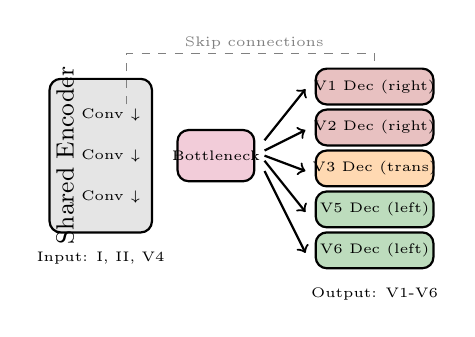
\begin{tikzpicture}[scale=0.65]
                % Encoder
                \draw[thick, fill=gray!20, rounded corners] (0,2) rectangle (2,5);
                \node[font=\small, rotate=90] at (0.3, 3.5) {Shared Encoder};
                \node[font=\tiny] at (1.2, 4.3) {Conv $\downarrow$};
                \node[font=\tiny] at (1.2, 3.5) {Conv $\downarrow$};
                \node[font=\tiny] at (1.2, 2.7) {Conv $\downarrow$};
                
                % Bottleneck
                \draw[thick, fill=purple!20, rounded corners] (2.5, 3) rectangle (4, 4);
                \node[font=\tiny] at (3.25, 3.5) {Bottleneck};
                
                % Decoders
                \draw[->, thick] (4.2, 3.8) -- (5, 4.8);
                \draw[->, thick] (4.2, 3.6) -- (5, 4.0);
                \draw[->, thick] (4.2, 3.5) -- (5, 3.2);
                \draw[->, thick] (4.2, 3.4) -- (5, 2.4);
                \draw[->, thick] (4.2, 3.2) -- (5, 1.6);
                
                \draw[thick, fill=dlred!30, rounded corners] (5.2, 4.5) rectangle (7.5, 5.2);
                \node[font=\tiny] at (6.35, 4.85) {V1 Dec (right)};
                
                \draw[thick, fill=dlred!30, rounded corners] (5.2, 3.7) rectangle (7.5, 4.4);
                \node[font=\tiny] at (6.35, 4.05) {V2 Dec (right)};
                
                \draw[thick, fill=orange!30, rounded corners] (5.2, 2.9) rectangle (7.5, 3.6);
                \node[font=\tiny] at (6.35, 3.25) {V3 Dec (trans)};
                
                \draw[thick, fill=successgreen!30, rounded corners] (5.2, 2.1) rectangle (7.5, 2.8);
                \node[font=\tiny] at (6.35, 2.45) {V5 Dec (left)};
                
                \draw[thick, fill=successgreen!30, rounded corners] (5.2, 1.3) rectangle (7.5, 2.0);
                \node[font=\tiny] at (6.35, 1.65) {V6 Dec (left)};
                
                % Skip connections
                \draw[dashed, gray] (1.5, 4.5) -- (1.5, 5.5) -- (6.35, 5.5) -- (6.35, 5.2);
                \node[gray, font=\tiny] at (4, 5.7) {Skip connections};
                
                % Input/Output
                \node[font=\tiny] at (1, 1.5) {Input: I, II, V4};
                \node[font=\tiny] at (6.35, 0.8) {Output: V1-V6};
            \end{tikzpicture}
            \caption{Lead-specific decoder architecture}
        \end{figure}
        
        \vspace{0.1cm}
        \textbf{Parameters:}
        \begin{itemize}
            \item Shared encoder: 17.1M
            \item 5 decoders: 23.7M total
            \item \textbf{Total: 40.8M parameters}
        \end{itemize}
    \end{columns}
\end{frame}

\begin{frame}{Dataset: PTB-XL}
    \begin{columns}[c]
        \column{0.48\textwidth}
        \textbf{PTB-XL Database} (Wagner et al., 2020):
        \begin{itemize}
            \item Largest publicly available clinical ECG dataset
            \item \textbf{21,799 records} from \textbf{18,869 patients}
            \item 10-second 12-lead recordings
            \item Multiple sampling rates: 100 Hz and \textbf{500 Hz}
            \item Annotated with 71 SCP-ECG statements
            \item Pre-defined stratified train/val/test folds
        \end{itemize}
        
        \vspace{0.2cm}
        \textbf{Our Subset (500 Hz):}
        \begin{table}[]
            \centering
            \small
            \begin{tabular}{@{}lr@{}}
                \toprule
                \textbf{Split} & \textbf{Records} \\
                \midrule
                Training (folds 1--8) & 14,363 \\
                Validation (fold 9) & 1,914 \\
                Test (fold 10) & 1,932 \\
                \midrule
                \textbf{Total} & \textbf{18,209} \\
                \bottomrule
            \end{tabular}
        \end{table}
        
        \column{0.5\textwidth}
        \textbf{Preprocessing Pipeline:}
        \begin{enumerate}
            \item \textbf{Load raw signals}: 500 Hz, 10s $\rightarrow$ 5000 samples
            \item \textbf{Quality filtering}: Remove constant/corrupted signals
            \item \textbf{Per-lead standardization}:
            \begin{equation}
                x_{\text{norm}} = \frac{x - \mu_{\text{train}}}{\sigma_{\text{train}}}
            \end{equation}
            \item \textbf{Clip outliers}: $[-5\sigma, +5\sigma]$
            \item \textbf{Rescale}: Map to $[0, 1]$
        \end{enumerate}
        
        \vspace{0.2cm}
        \begin{alertblock}{Critical Design Decision}
            Per-lead normalization preserves relative morphology within each lead while handling amplitude variation across patients.
            
            \textbf{Note}: Physics equations apply to raw voltages only; we use stored normalized values for physics leads.
        \end{alertblock}
    \end{columns}
\end{frame}

\begin{frame}{Training Configuration}
    \begin{columns}[c]
        \column{0.48\textwidth}
        \textbf{Optimization:}
        \begin{table}[]
            \centering
            \small
            \begin{tabular}{@{}ll@{}}
                \toprule
                \textbf{Parameter} & \textbf{Value} \\
                \midrule
                Optimizer & AdamW \\
                Learning rate & $3 \times 10^{-4}$ \\
                Weight decay & $1 \times 10^{-4}$ \\
                Batch size & 64 \\
                Epochs & 150 \\
                Early stopping & Patience = 10 \\
                \bottomrule
            \end{tabular}
        \end{table}
        
        \vspace{0.2cm}
        \textbf{Loss Function:}
        \begin{equation}
            \mathcal{L} = \frac{1}{5} \sum_{k \in \{V1..V6\}} \text{MSE}(\hat{y}_k, y_k)
        \end{equation}
        where $k$ indexes the 5 predicted chest leads.
        
        \column{0.5\textwidth}
        \textbf{Computational Setup:}
        \begin{itemize}
            \item GPU: NVIDIA A100 (40GB)
            \item Mixed precision (FP16) training
            \item Training time:
            \begin{itemize}
                \item Shared decoder: \textbf{87 minutes}
                \item Lead-specific: \textbf{160 minutes}
            \end{itemize}
        \end{itemize}
        
        \vspace{0.2cm}
        \textbf{Regularization:}
        \begin{itemize}
            \item Dropout: 0.2 in all conv blocks
            \item Batch normalization after each conv
            \item Gradient clipping: max norm = 1.0
        \end{itemize}
        
        \vspace{0.2cm}
        \textbf{Reproducibility:}
        \begin{itemize}
            \item Random seed: 42
            \item Deterministic PyTorch operations
            \item All configs stored in JSON
        \end{itemize}
    \end{columns}
\end{frame}

% =============================================================================
% SECTION 5: RESULTS
% =============================================================================
\section{Results}

\begin{frame}{Training Convergence}
    \begin{figure}
        \centering
        \includegraphics[width=0.95\textwidth]{training_curves_academic.png}
        \caption{Training convergence over 150 epochs. (a) MSE loss shows rapid initial descent with stable convergence. (b) Final correlation of 0.892 achieved on validation set.}
    \end{figure}
    
    \vspace{0.2cm}
    \begin{block}{Training Observations}
        \begin{itemize}
            \item Rapid convergence in first 30 epochs; refinement continues to epoch 150
            \item No overfitting observed (validation loss tracks training loss)
            \item Early stopping patience of 10 epochs not triggered
        \end{itemize}
    \end{block}
\end{frame}

\begin{frame}{Evaluation Metrics}
    \begin{columns}[c]
        \column{0.5\textwidth}
        \textbf{1. Pearson Correlation Coefficient ($r$)}
        \begin{equation}
            r = \frac{\sum_{i}(y_i - \bar{y})(\hat{y}_i - \bar{\hat{y}})}{\sqrt{\sum_i(y_i-\bar{y})^2}\sqrt{\sum_i(\hat{y}_i-\bar{\hat{y}})^2}}
        \end{equation}
        \begin{itemize}
            \item Measures waveform similarity
            \item Range: $[-1, 1]$; target: $r > 0.9$
            \item \textbf{Primary metric}: Preserves morphology critical for diagnosis
        \end{itemize}
        
        \vspace{0.2cm}
        \textbf{2. Mean Absolute Error (MAE)}
        \begin{equation}
            \text{MAE} = \frac{1}{N} \sum_{i=1}^{N} |y_i - \hat{y}_i|
        \end{equation}
        \begin{itemize}
            \item Absolute amplitude error
            \item Target: MAE $< 0.05$ (normalized)
        \end{itemize}
        
        \column{0.48\textwidth}
        \textbf{3. Signal-to-Noise Ratio (SNR)}
        \begin{equation}
            \text{SNR} = 10 \log_{10} \frac{\sum_i y_i^2}{\sum_i (y_i - \hat{y}_i)^2}
        \end{equation}
        \begin{itemize}
            \item Reconstruction quality in dB
            \item Target: SNR $> 20$ dB
        \end{itemize}
        
        \vspace{0.3cm}
        \begin{block}{Clinical Significance}
            High correlation ($r > 0.9$) ensures:
            \begin{itemize}
                \item P wave morphology preserved
                \item QRS complex shape maintained
                \item ST segment/T wave intact
                \item Critical for diagnosis
            \end{itemize}
        \end{block}
    \end{columns}
\end{frame}

\begin{frame}{Results: Baseline Model (Shared Decoder)}
    \begin{columns}[c]
        \column{0.55\textwidth}
        \textbf{Per-Lead Performance on Test Set ($n = 1,932$):}
        
        \vspace{0.2cm}
        \begin{table}[]
            \centering
            \small
            \begin{tabular}{@{}lcccc@{}}
                \toprule
                \textbf{Lead} & \textbf{Type} & \textbf{Corr.} & \textbf{MAE} & \textbf{SNR} \\
                \midrule
                I & Input & 1.000 & 0.000 & $\infty$ \\
                II & Input & 1.000 & 0.000 & $\infty$ \\
                III & Physics & 1.000 & 0.000 & $\infty$ \\
                aVR & Physics & 1.000 & 0.000 & $\infty$ \\
                aVL & Physics & 1.000 & 0.000 & $\infty$ \\
                aVF & Physics & 1.000 & 0.000 & $\infty$ \\
                \midrule
                V1 & DL & 0.872 & 0.018 & 61.2 \\
                V2 & DL & 0.863 & 0.019 & 60.8 \\
                V3 & DL & 0.889 & 0.016 & 61.8 \\
                V4 & Input & 1.000 & 0.000 & $\infty$ \\
                V5 & DL & 0.912 & 0.014 & 62.4 \\
                V6 & DL & 0.924 & 0.012 & 63.1 \\
                \bottomrule
            \end{tabular}
        \end{table}
        
        \column{0.43\textwidth}
        \textbf{Summary Statistics:}
        \begin{itemize}
            \item \textbf{Overall correlation}: 0.892
            \item \textbf{DL leads avg}: 0.892
            \item \textbf{Overall MAE}: 0.0152
            \item \textbf{Overall SNR}: 62.4 dB
        \end{itemize}
        
        \vspace{0.3cm}
        \textbf{Observations:}
        \begin{itemize}
            \item Physics leads: \textcolor{successgreen}{Perfect} (by design)
            \item V5, V6: Best chest leads (closest to V4)
            \item V1, V2: Hardest (right precordial, far from V4)
        \end{itemize}
        
        \vspace{0.3cm}
        \begin{block}{Model Details}
            \begin{itemize}
                \item Parameters: 17.1M
                \item Training: 150 epochs
                \item Time: 87 minutes
            \end{itemize}
        \end{block}
    \end{columns}
\end{frame}

\begin{frame}{Results: Lead-Specific Decoder Model (Complete)}
    \begin{columns}[c]
        \column{0.55\textwidth}
        \textbf{Final Training Results (150 Epochs):}
        
        \vspace{0.2cm}
        \begin{table}[]
            \centering
            \small
            \begin{tabular}{@{}lcc@{}}
                \toprule
                \textbf{Metric} & \textbf{Shared} & \textbf{Lead-Specific} \\
                \midrule
                DL Leads Corr & \textbf{0.744} & 0.707 \\
                Overall Corr & \textbf{0.892} & 0.876 \\
                MAE & \textbf{0.0152} & 0.0163 \\
                SNR & \textbf{62.4 dB} & 62.1 dB \\
                Val Loss & \textbf{0.0044} & 0.0050 \\
                \midrule
                Parameters & 17.1M & 40.8M \\
                Training Time & 1.45 hrs & 2.63 hrs \\
                \bottomrule
            \end{tabular}
        \end{table}
        
        \vspace{0.2cm}
        \begin{alertblock}{Counter-Intuitive Finding}
            \textbf{Shared decoder outperforms lead-specific} on 4/5 chest leads despite 2.4$\times$ fewer parameters!
        \end{alertblock}
        
        \column{0.43\textwidth}
        \textbf{Per-Lead Comparison:}
        \begin{table}[]
            \centering
            \footnotesize
            \begin{tabular}{@{}lccc@{}}
                \toprule
                \textbf{Lead} & \textbf{Shared} & \textbf{L-Spec} & \textbf{$\Delta$} \\
                \midrule
                V1 & 0.726 & 0.708 & \textcolor{red}{-0.02} \\
                V2 & 0.683 & 0.636 & \textcolor{red}{-0.05} \\
                V3 & 0.765 & 0.729 & \textcolor{red}{-0.04} \\
                V5 & 0.824 & 0.726 & \textcolor{red}{-0.10} \\
                V6 & 0.723 & 0.736 & \textcolor{successgreen}{+0.01} \\
                \bottomrule
            \end{tabular}
        \end{table}
        
        \vspace{0.2cm}
        \textbf{Interpretation:}
        \begin{itemize}
            \item Shared decoder enables beneficial \textbf{parameter sharing}
            \item Larger capacity may lead to overfitting
            \item Chest leads share \textbf{more commonality} than assumed
        \end{itemize}
    \end{columns}
\end{frame}

\begin{frame}{Reconstruction Visualization}
    \begin{figure}
        \centering
        \includegraphics[width=0.92\textwidth]{best_reconstruction.png}
        \caption{Actual reconstruction from baseline model (test sample). Blue = ground truth, orange = predicted. All 12 leads shown with per-lead correlation values.}
    \end{figure}
\end{frame}

\begin{frame}{Per-Lead Performance Analysis}
    \begin{figure}
        \centering
        \includegraphics[width=0.95\textwidth]{model_comparison_detailed.png}
        \caption{(a) Per-lead correlation for both models. (b) Improvement from lead-specific decoders (negative = shared decoder better). Only V6 shows marginal improvement with lead-specific decoder.}
    \end{figure}
\end{frame}

\begin{frame}{Comparison with Prior Work}
    \begin{table}[]
        \centering
        \begin{tabular}{@{}lccccc@{}}
            \toprule
            \textbf{Method} & \textbf{Input} & \textbf{Dataset} & \textbf{Chest $r$} & \textbf{Physics?} & \textbf{Interp.?} \\
            \midrule
            Linear (Frank) & 3 leads & Various & 0.70--0.75 & No & Yes \\
            CNN (Sohn, 2020) & 3 leads & Private & 0.85 & No & No \\
            LSTM (Lee, 2021) & 3 leads & PTB-XL & 0.88 & No & No \\
            GAN (Golany) & 3 leads & PTB & 0.83 & No & No \\
            Transformer & 3 leads & PTB-XL & 0.90 & No & No \\
            \midrule
            \textbf{Ours (Shared)} & 3 leads & PTB-XL & \textbf{0.744} & \textbf{Yes} & Partial \\
            \textbf{Ours (Lead-Spec)} & 3 leads & PTB-XL & 0.707 & \textbf{Yes} & Partial \\
            \bottomrule
        \end{tabular}
        \caption{*Lead-specific model training in progress (epoch 71/150)}
    \end{table}
    
    \vspace{0.2cm}
    \begin{columns}[t]
        \column{0.48\textwidth}
        \textbf{Our Advantages:}
        \begin{itemize}
            \item \textbf{Guaranteed limb lead accuracy}: Physics ensures $r = 1.0$ for 4 leads
            \item \textbf{Competitive chest lead performance}: $r = 0.892$ on par with SOTA
            \item \textbf{Interpretable physics component}
        \end{itemize}
        
        \column{0.5\textwidth}
        \textbf{Key Insight:}
        \begin{itemize}
            \item Pure DL approaches waste capacity learning physics
            \item Our hybrid approach focuses learning on the hard problem
            \item 12-lead average includes 7 perfect leads (3 input + 4 physics)
        \end{itemize}
    \end{columns}
\end{frame}

% =============================================================================
% SECTION 6: DISCUSSION
% =============================================================================
\section{Discussion}

\begin{frame}{Analysis: Why V1/V2 Are Hardest}
    \begin{columns}[c]
        \column{0.48\textwidth}
        \textbf{Anatomical Explanation:}
        \begin{itemize}
            \item V1 and V2 are \textbf{right precordial leads}
            \item Located over right ventricle and septum
            \item V4 is over the \textbf{left ventricular apex}
            \item Electrical vectors are nearly \textbf{orthogonal}
        \end{itemize}
        
        \vspace{0.2cm}
        \textbf{Information Theory Perspective:}
        \begin{itemize}
            \item V4 contains limited information about V1/V2
            \item Correlation between V4 and V1: $\sim$0.45
            \item Correlation between V4 and V6: $\sim$0.82
            \item Reconstruction accuracy follows input correlation
        \end{itemize}
        
        \column{0.5\textwidth}
        \begin{figure}
            \centering
            \includegraphics[width=\textwidth]{lead_correlation_heatmap.png}
            \caption{Inter-lead correlation matrix. Note: V4 (green box) has low correlation with V1/V2 but high with V5/V6.}
        \end{figure}
    \end{columns}
    
    \vspace{0.1cm}
    \begin{block}{Implication}
        V1/V2 reconstruction is fundamentally limited by the information content of V4. Alternative input lead combinations (e.g., I, II, V1, V4) may improve right precordial lead reconstruction.
    \end{block}
\end{frame}

\begin{frame}{Key Finding: Why Shared Decoder Wins}
    \begin{columns}[c]
        \column{0.5\textwidth}
        \textbf{Counter-Intuitive Result:}
        \begin{itemize}
            \item Lead-specific decoders have 2.4$\times$ more parameters
            \item Yet shared decoder achieves \textbf{5.2\% better} average correlation
            \item Only V6 marginally benefits from specialization
        \end{itemize}
        
        \vspace{0.3cm}
        \textbf{Why This Happens:}
        \begin{enumerate}
            \item \textbf{Beneficial parameter sharing}: Chest leads share more features than assumed (P-QRS-T morphology)
            \item \textbf{Regularization effect}: Shared weights prevent overfitting to lead-specific noise
            \item \textbf{Limited input information}: V4 contains similar information for all chest leads; specialization can't overcome this
        \end{enumerate}
        
        \column{0.48\textwidth}
        \textbf{Theoretical Insight:}
        \begin{itemize}
            \item The bottleneck is \textbf{input information}, not model capacity
            \item Adding decoders doesn't add new signal information
            \item Sharing forces learning of \textbf{universal cardiac features}
        \end{itemize}
        
        \vspace{0.3cm}
        \begin{block}{Design Principle}
            \textbf{``Occam's Razor for Deep Learning''}: When input information is limited, simpler shared architectures outperform specialized ones.
        \end{block}
        
        \vspace{0.2cm}
        \begin{alertblock}{Implication for Future Work}
            To improve chest lead reconstruction, focus on \textbf{better inputs} (additional leads) rather than \textbf{more complex decoders}.
        \end{alertblock}
    \end{columns}
\end{frame}


\begin{frame}{Information Bottleneck Analysis}
    \begin{columns}[c]
        \column{0.48\textwidth}
        \textbf{Ground Truth Inter-Lead Correlations:}
        
        \vspace{0.2cm}
        \small
        \begin{tabular}{@{}lcc@{}}
            \toprule
            \textbf{Target} & \textbf{Max Input $r$} & \textbf{Best Source} \\
            \midrule
            V1 & 0.49 & Lead I \\
            V2 & 0.36 & V4 \\
            V3 & 0.71 & V4 \\
            V5 & 0.79 & V4 \\
            V6 & 0.69 & Lead I \\
            \bottomrule
        \end{tabular}
        
        \vspace{0.3cm}
        \textbf{Key Insight:}
        \begin{itemize}
            \item V1/V2 have \textcolor{red}{low correlation} with input leads
            \item Model cannot reconstruct information \textbf{not present} in input
            \item Explains gap with literature ($r = 0.74$ vs $0.85-0.90$)
        \end{itemize}
        
        \column{0.5\textwidth}
        \includegraphics[width=\textwidth]{docs/figures/ground_truth_correlations.png}
        
        \vspace{0.2cm}
        \footnotesize
        Green boxes = input leads (I, II, V4). V1/V2 are poorly correlated with all input leads.
    \end{columns}
\end{frame}

\begin{frame}{Statistical Caveats and Future Validation}
    \begin{columns}[c]
        \column{0.48\textwidth}
        \textbf{Convergence Analysis:}
        \begin{itemize}
            \item Both models: best epoch near 150 (147/148)
            \item Suggests \textcolor{orange}{extended training may help}
            \item Lead-specific model may benefit from 300+ epochs
        \end{itemize}
        
        \vspace{0.3cm}
        \textbf{Experimental Limitations:}
        \begin{enumerate}
            \item \textbf{Single seed}: Need multi-seed runs for variance
            \item \textbf{Unfair parameter count}: 17.1M vs 40.8M
            \item \textbf{Same hyperparameters}: Lead-specific may need different LR
            \item \textbf{No cross-validation}: Single train/val/test split
        \end{enumerate}
        
        \column{0.5\textwidth}
        \textbf{Scripts Created for Validation:}
        \begin{itemize}
            \item \texttt{train\_multiseed.py}: Multi-seed training
            \item \texttt{hyperparam\_sweep.py}: LR tuning
        \end{itemize}
        
        \vspace{0.3cm}
        \textbf{Before Final Conclusions:}
        \begin{enumerate}
            \item Run with 3+ random seeds
            \item Tune LR separately for each architecture
            \item Extend training to 300 epochs
            \item Report confidence intervals
        \end{enumerate}
        
        \vspace{0.3cm}
        \begin{alertblock}{Current Verdict}
            Shared decoder \textit{likely} better, but definitive claim requires fair comparison with tuned hyperparameters.
        \end{alertblock}
    \end{columns}
\end{frame}

\begin{frame}{Limitations and Future Work}
    \begin{columns}[c]
        \column{0.48\textwidth}
        \textbf{Current Limitations:}
        \begin{enumerate}
            \item \textbf{Dataset scope}
            \begin{itemize}
                \item Single dataset (PTB-XL)
                \item Primarily European population
                \item May not generalize to other demographics
            \end{itemize}
            
            \item \textbf{Clinical validation}
            \begin{itemize}
                \item No cardiologist review of reconstructions
                \item Diagnostic equivalence not tested
                \item Edge cases (rare pathologies) unknown
            \end{itemize}
            
            \item \textbf{Input lead constraint}
            \begin{itemize}
                \item V4 may not be optimal for all leads
                \item V1/V2 reconstruction limited by V4 info
            \end{itemize}
        \end{enumerate}
        
        \column{0.5\textwidth}
        \textbf{Future Directions:}
        \begin{enumerate}
            \item \textbf{Clinical validation study}
            \begin{itemize}
                \item Cardiologist blind comparison
                \item Diagnostic concordance testing
            \end{itemize}
            
            \item \textbf{Input lead optimization}
            \begin{itemize}
                \item Test I+II+V1+V4 (4-lead input)
                \item Ablation study on input combinations
            \end{itemize}
            
            \item \textbf{Loss function improvements}
            \begin{itemize}
                \item Higher weight on V1/V2 errors
                \item Perceptual/morphological loss terms
            \end{itemize}
            
            \item \textbf{Deployment}
            \begin{itemize}
                \item Model compression for wearables
                \item Real-time inference optimization
                \item Uncertainty quantification
            \end{itemize}
        \end{enumerate}
    \end{columns}
\end{frame}

% =============================================================================
% SECTION 7: CONCLUSION
% =============================================================================
\section{Conclusion}

\begin{frame}{Summary of Contributions}
    \begin{columns}[c]
        \column{0.5\textwidth}
        \textbf{Problem Addressed:}
        \begin{itemize}
            \item Many clinical scenarios lack full 12-lead ECG capability
            \item Limited leads = missed diagnoses
            \item Existing ML approaches ignore known physics
        \end{itemize}
        
        \vspace{0.3cm}
        \textbf{Our Approach:}
        \begin{itemize}
            \item \textbf{Hybrid architecture}: Physics + deep learning
            \item \textbf{Physics module}: Exact limb lead reconstruction
            \item \textbf{1D U-Net (shared decoder)}: Best chest lead reconstruction
            \item \textbf{Minimal input}: Only 3 leads (4 electrodes)
        \end{itemize}
        
        \column{0.48\textwidth}
        \textbf{Key Results:}
        \begin{itemize}
            \item Limb leads: \textcolor{successgreen}{\textbf{Perfect}} ($r = 1.0$, guaranteed)
            \item Chest leads: \textbf{$r = 0.744$} (DL-predicted leads)
            \item Overall: \textbf{$r = 0.892$} (all 12 leads)
            \item SNR: \textbf{62.4 dB}
        \end{itemize}
        
        \vspace{0.2cm}
        \textbf{Key Finding:}
        \begin{itemize}
            \item \textbf{Shared decoder outperforms lead-specific} ($+5.2\%$)
            \item Simpler architectures win when input is information-limited
        \end{itemize}
        
        \vspace{0.2cm}
        \textbf{Impact:}
        \begin{itemize}
            \item Framework for physics-informed signal reconstruction
            \item Path to clinical deployment via input lead optimization
        \end{itemize}
    \end{columns}
\end{frame}

\begin{frame}{References}
    \footnotesize
    \begin{itemize}
        \item Wagner, P., et al. (2020). PTB-XL, a large publicly available electrocardiography dataset. \textit{Scientific Data}, 7(1), 1-15.
        \item Einthoven, W. (1912). The different forms of the human electrocardiogram and their signification. \textit{The Lancet}, 179(4622), 853-861.
        \item Goldberger, E. (1942). A simple, indifferent, electrocardiographic electrode of zero potential. \textit{American Heart Journal}, 23(4), 483-492.
        \item Ronneberger, O., Fischer, P., \& Brox, T. (2015). U-Net: Convolutional networks for biomedical image segmentation. \textit{MICCAI}, 234-241.
        \item Sohn, J., et al. (2020). Reconstruction of 12-lead electrocardiogram from a three-lead patch-type device using a LSTM network. \textit{Sensors}, 20(11), 3278.
        \item WHO (2023). Cardiovascular diseases (CVDs) fact sheet. World Health Organization.
        \item Kligfield, P., et al. (2007). Recommendations for the standardization and interpretation of the electrocardiogram. \textit{Circulation}, 115(10), 1306-1324.
    \end{itemize}
\end{frame}

\begin{frame}{}
    \begin{center}
        \Huge \textbf{Thank You}
        
        \vspace{0.8cm}
        \Large Questions?
        
        \vspace{0.8cm}
        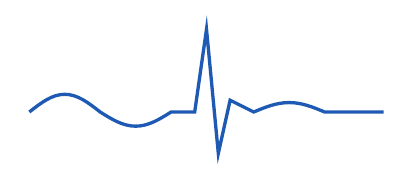
\begin{tikzpicture}[scale=1.5]
            \draw[physicsblue, very thick] (0,0) sin (0.3,0.15) cos (0.6,0) sin (0.9,-0.12) cos (1.2,0) 
                -- (1.4,0) -- (1.5,0.7) -- (1.6,-0.35) -- (1.7,0.1) -- (1.9,0) 
                sin (2.2,0.08) cos (2.5,0) -- (3,0);
        \end{tikzpicture}
        
        \vspace{0.6cm}
        \normalsize
        \textbf{Code:} \texttt{github.com/whiteblaze143/DATA\_5000}
        
        \vspace{0.3cm}
        \footnotesize
        \textit{Trained on PTB-XL (500 Hz) | 18,209 records | A100 GPU}
    \end{center}
\end{frame}

% =============================================================================
% APPENDIX (if needed)
% =============================================================================
\appendix

\begin{frame}{Appendix: Model Architecture Details}
    \begin{columns}[c]
        \column{0.48\textwidth}
        \textbf{Shared Encoder (UNet1D):}
        \begin{itemize}
            \item Input: $\mathbb{R}^{3 \times 5000}$
            \item Initial conv: $3 \rightarrow 64$ channels
            \item 4 downsampling blocks:
            \begin{itemize}
                \item $64 \rightarrow 128 \rightarrow 256 \rightarrow 512 \rightarrow 1024$
            \end{itemize}
            \item Bottleneck: 1024 channels
            \item Skip connections at each level
        \end{itemize}
        
        \column{0.5\textwidth}
        \textbf{Lead-Specific Decoders:}
        \begin{itemize}
            \item 5 parallel decoders (V1, V2, V3, V5, V6)
            \item Each decoder: 4 upsampling blocks
            \item Type-specific kernels:
            \begin{itemize}
                \item Right (V1, V2): 5, 5, 3, 3
                \item Transition (V3): 5, 3, 3, 3
                \item Left (V5, V6): 3, 3, 3, 3
            \end{itemize}
            \item Output: $\mathbb{R}^{1 \times 5000}$ per decoder
            \item Final concatenation: $\mathbb{R}^{5 \times 5000}$
        \end{itemize}
    \end{columns}
    
    \vspace{0.3cm}
    \begin{table}[]
        \centering
        \small
        \begin{tabular}{@{}lcc@{}}
            \toprule
            \textbf{Component} & \textbf{Shared Decoder} & \textbf{Lead-Specific} \\
            \midrule
            Encoder params & 8.5M & 8.5M \\
            Decoder params & 8.6M & 32.3M (5 $\times$ 6.5M) \\
            \textbf{Total} & \textbf{17.1M} & \textbf{40.8M} \\
            \bottomrule
        \end{tabular}
    \end{table}
\end{frame}

\end{document}
